\chapter{Introduction}

Le but de se projet est de mettre en place une chaine décisionnelle. L'objectif de ce projet n'étant pas de pousser dans ses retranchements les outils de la chaine décisionnelle, il a été décidé de créer de toute pièce un jeu de données. Le thème de ce jeu de données est l'achat de BD comme dans le cours. 
La base opérationnelle décrit les factures d'un ensemble librairies en France dont les clients sont connus.
La chaine décisionnelle doit être en mesure de répondre in fine à la question: analyser les ventes de BD en France en fonction des clients, du lieu et date d'achat.
La couche opérationnelle est assurée par une base de données de fichier csv et une base de données PostgresSQL. 

Pour la couche ETL, il a été choisi TALEND Data Integration. 

La couche reporting étudiée lors de ce projet est assurée par SAS Studio Version Etudiante.


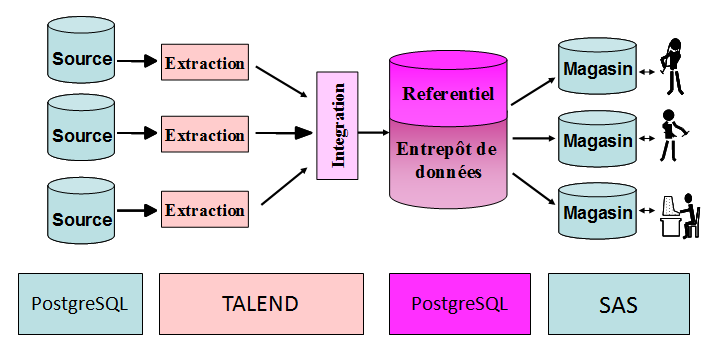
\includegraphics[clip=true, width=120mm, height=80mm]{images/chaine.png} 
\label{chaine}



\clearpage
